%&latex
\documentclass[12pt]{article}
\usepackage{amsmath}
\usepackage{graphicx}
\usepackage{float}
\usepackage{tikz}
\usetikzlibrary{shapes.geometric, arrows}
\usepackage{enumerate}
\usepackage{natbib}
\usepackage{url}
\usepackage{caption}


\setlength{\abovedisplayskip}{5pt}  % Reduce space above equations
\setlength{\belowdisplayskip}{5pt} 

% Define block styles
\tikzstyle{startstop} = [rectangle, rounded corners, minimum width=3cm, minimum height=1cm,text centered, draw=black, fill=red!30]
\tikzstyle{process} = [rectangle, minimum width=3cm, minimum height=1cm, text centered, draw=black, fill=blue!30]
\tikzstyle{decision} = [diamond, minimum width=3cm, minimum height=1cm, text centered, draw=black, fill=green!30]
\tikzstyle{arrow} = [thick,->,>=stealth]

%\pdfminorversion=4
% NOTE: To produce blinded version, replace "0" with "1" below.
\newcommand{\blind}{0}

% DON'T change margins - should be 1 inch all around.
\addtolength{\oddsidemargin}{-.5in}%
\addtolength{\evensidemargin}{-.5in}%
\addtolength{\textwidth}{1in}%
\addtolength{\textheight}{1.3in}%
\addtolength{\topmargin}{-.8in}%


\begin{document}

%\bibliographystyle{natbib}

\def\spacingset#1{\renewcommand{\baselinestretch}%
{#1}\small\normalsize} \spacingset{1}


%%%%%%%%%%%%%%%%%%%%%%%%%%%%%%%%%%%%%%%%%%%%%%%%%%%%%%%%%%%%%%%%%%%%%%%%%%%%%%

\if0\blind
{
  \title{\bf Advancements in Health Prediction Using Machine Learning
Techniques(Heart Disease Prediction)}
  \author{Yashwanth Kotha\hspace{.2cm}\\
    Department of Data Science, University at Albany, SUNY\\
    }
  \maketitle
} \fi

\if1\blind
{
  \bigskip
  \bigskip
  \bigskip
  \begin{center}
    {\LARGE\bf Title}
\end{center}
  \medskip
} \fi

\bigskip
\begin{abstract}
The World Health Organization estimates that by 2030, cardiovascular diseases (CVDs) would account for 23.6 million deaths worldwide, making it one of the major causes of death. Particularly after the COVID-19 epidemic, the cases of CVDs has dramatically increased in recent years, underscoring the importance of early detection and prevention. Using a dataset of 70,000 medical records with 13 features—including age, blood sugar, cholesterol,smoking, and alcohol—this study investigates the application of machine learning techniques to predict cardiac disease. The dataset was preprocessed in order to remove outliers and generate additional features such as Mean Arterial Pressure (MAP) and Body Mass Index (BMI). Machine learning models like Logistic Regression, Random Forest, and Naïve Bayes were trained and evaluated using performance metrics including accuracy, recall, precision, and ROC-AUC scores. The results highlight machine learning's promise in healthcare, especially for early at-risk individual identification. These prediction models highlight the significance of incorporating sophisticated analytics into preventive healthcare initiatives by enabling prompt interventions that can enhance patient outcomes and greatly lessen the effect of cardiovascular illnesses.



\end{abstract}

\noindent%
{\it Keywords:}  Dataset, Machine learning models, Features, Accuracy, ROC-AUC
\vfill

\newpage
\tableofcontents
\newpage

\spacingset{1.45} % DON'T change the spacing!
\section{Introduction}
The goal of this study is to forecast heart disease by analyzing medical data and identifying people who are at risk using machine learning techniques. I have used 13 features from a dataset of 70,000 entries, which included patient characteristics including age, blood sugar, cholesterol, and lifestyle choices. In order to improve feature representation and eliminate outliers, the data was preprocessed. This included the development of new metrics such as Mean Arterial Pressure (MAP) and Body Mass Index (BMI).

I  used machine learning classifiers like Naïve Bayes, Random Forest, and Logistic Regression to construct the prediction model. To ascertain how well these models performed in correctly identifying people as having or not having heart disease, they were trained and validated. Out of all the studied algorithms, Logistic Regression proved to be the most successful model, attaining the maximum accuracy.

In order to comprehend the connections between risk variables and cardiovascular diseases, I have also involved statistical testing, exploratory data analysis, and visualizations. This research serves as an example of how data-driven methods can help prevent and detect heart disease early, leading to better health outcomes.
\section{Literature Survey}
\label{sec:intro}

This review aims to analyze the effectiveness of different machine learning approaches in heart disease prediction, focusing on their performance, accuracy, and potential for real-world health care applications. The journals reviewed in this study focus on using machine learning algorithms to enhance heart disease diagnosis.



\begin{itemize}
\setlength{\itemsep}{0pt}  % Removes extra space between items
  \setlength{\parskip}{0pt}
\item \textbf{Sharma et al. (2020)} study uses machine learning to predict heart disease based on the UCI Heart Disease dataset, a popular dataset containing 14 attributes like age, gender, and cholesterol levels. The researchers applied several machine learning models, including Random Forest, SVM, Naive Bayes, and Decision Tree. Random Forest performed best in this study, achieving high accuracy by handling noise in the data well and avoiding overfitting. This study suggests that Random Forest could be a reliable choice for predicting heart disease because it balances accuracy with stability in prediction.


\item \textbf{Kavitha et al. (2021)} paper explores a hybrid approach, which combines Decision Tree and Random Forest models for heart disease prediction. Using the Cleveland Heart Disease dataset, which includes similar health attributes, the study achieved an accuracy rate of 88.7\% with the hybrid model. The authors argue that combining models, known as a hybrid approach, can capture different patterns in the data, leading to better predictions. They also created an interface where users could enter their information, and the model would predict their risk. This approach is useful in real-time applications and highlights how model combinations can enhance prediction reliability.




\begin{table}[H]
\caption{UCI Dataset  \label{tab:tabone}}
\begin{center}
\small
\begin{tabular}{cccc}
S. No. & Attribute & Description & Mean \\\hline
1 & Age & in years & 54.434 \\
2 & Sex & Male, Female & 0.696 \\
3 & CP & Angina, Abnang, Notang, Asympt & 0.942 \\
4 & TestBPS & Resting bp in mm hg &  131.612\\
5 & Chol  & Serum Cholestrol in mg/dl & 246 \\
6 & FBS & Fasting blood sugar &  0.149\\
7 & RestECG & Electrocardiographic Results &  0.53\\
8 & Thalach & Maximum Heart rate observed &  149.114\\
9 & Exang & Exercise with angina has occured &  0.337\\
10 & Olpeak & ST depression induced through exercise & 1.072 \\
11 & Slope & Slope of the ST segment &  1.385\\
12 & Thal & Number of major vessels &  0.754\\
12 & CA & Heart Status &  2.34\\
12 & Target & Output Class &  \\

\end{tabular}
\end{center}
\end{table}



\item \textbf{Senthilkumar Mohan et al. (2019)} paper explores on machine learning models like Decision tree, Language model, Support vector machine, Random forest, Naïve Bayes, Neural Networks, and K-Nearest Neighbour. Out of all these models combination of Random forest and Linear method gave the best accuracy in predicting heart
disease for the given datset.


\item \textbf{Bhatt et al. (2023)} focused on increasing prediction accuracy by applying various models, such as Decision Tree, Random Forest, Multilayer Perceptron, and XGBoost, on a large dataset of 70,000 entries. The dataset included key health metrics like blood pressure, cholesterol levels, and glucose levels. Among the tested models, the Multilayer Perceptron performed best, reaching an best accuracy after tuning the model’s parameters. The authors conclude that a larger dataset can help the model learn more general patterns, improving the accuracy and making it more applicable across different populations 


\item \textbf{Ramalingam et al. (2018)} paper reviewed several machine learning techniques used for predicting heart disease. Models like SVM, KNN, Naive Bayes, Decision Tree, and Random Forest were discussed, focusing on how they work with medical data. The authors emphasize that reducing the number of features, a process known as dimensionality reduction, can improve model performance by removing unnecessary information. They highlight techniques like Principal Component Analysis (PCA) and Chi-square tests, which help select the most important features and avoid model overfitting, a problem where the model fails to generalize to new data.




\item \textbf{Jindal et al. (2021)} tested three main algorithms: Logistic Regression, KNN, and Random Forest, on the UCI Heart Disease dataset. They found that KNN (K-Nearest Neighbors) achieved the highest accuracy, slightly outperforming the other methods. The authors suggest that using more than one algorithm for training could improve the final results. They also emphasize the importance of data pre-processing, such as cleaning and organizing the data before training, to improve model accuracy
and efficiency


\item \textbf{Samir Patel et al. (2016)} paper has tested three main algorithms: J48, Logistic Model Tree, and Random Forest Algorithm. From these three, J48 model turned out to be best classifier for heart disease prediction because it contains more accuracy and least total time to build.

\item \textbf{Jagtap et al. (2019)} study uses machine learning to predict heart disease based on the machine learning models like Support Vector Machine, Logistic regression, and Naïve Bayes Algorithm. This study suggests that SVM could be a reliable choice for predicting heart disease because it balances accuracy with stability in prediction


\item \textbf{Aditi et al. (2018)} used MLP Classifier for predicting heart disease using machine learning models. MLP provides its users with a prediction result that gives the state of a user leading to CAD. It says that they have used MLP in the proposed system because of its efficiency and accuracy. Also, the algorithm gives the nearby reliable output based on the input provided by the users.


\item \textbf{Archana et al. (2020)} examined the accuracy of algorithms like K-Nearest Neighbors, Decision Trees, Linear Regression, and SVM in predicting heart diseases. The study utilizes the UCI repository dataset and evaluates models based on training and testing performance. Machine learning algorithms prove to be efficient in early disease detection, with the Decision Tree model noted for its high accuracy. This work underlines the potential of supervised learning methods in improving health outcomes through reliable and early prediction.

\end{itemize}

\section{Existing Methodologies}
\label{sec:meth}
Models used in different papers are listed below,
\begin{itemize}
\setlength{\itemsep}{0pt}  % Removes extra space between items
  \setlength{\parskip}{0pt}
\item \textbf{Logistic regression} \\
 Logistic regression is used to find the
relationships between two data factors.  It is a binary classifier, usually has a finite number of outcomes, like yes or no. The logistic function maps the dependent variable as a sigmoid function of the independent variable, resulting in an S-curve. The function returns values between 0 and 1 for the dependent variable, regardless of the independent variable values.
\begin{equation}
p(y = 1 | x) = \frac{1}{1 + e^{-(w_0 + \sum_{i=1}^{n} w_i x_i)}}
\end{equation}

where \( p(y = 1 | x) \) is the probability of the positive class, \( w_0 \) is the bias term, \( w_i \) are the weights, and \( x_i \) are the input features. The function uses the sigmoid function to output values between 0 and 1.

 
 
\item \textbf{Decision tree} \\
For classification and regression applications, a decision tree is a model that resembles a tree. Based on feature values, it divides the dataset into branches, making decisions at each node until it reaches a final classification at the leaf nodes. Decision trees are a common option in medical diagnostics because they are simple to analyze and comprehend. They are susceptible to overfitting, nevertheless, particularly when dealing with noisy data. Pruning is one technique that is frequently used to improve the model's performance.
\begin{equation}
H(D) = - \sum_{j=1}^{m} p_j \log_2 p_j
\end{equation}

where:
$H(D)$ is the entropy of dataset $D$, $m$ is the number of classes, and $p_j$ is the proportion of instances belonging to class $j$.



\item \textbf{Random Forest} \\
It is a collection of decision trees. Bagging technique is used to build a random forest algorithm. This means that each decision tree in the forest is trained on a random subset of the training data, sampled with replacement, thereby producing diverse trees that, when combined, contribute to a more robust prediction. The final prediction is calculated by combining the predictions from each decision tree. The algorithm is well-suited for complicated tasks like the prediction of heart disease because it can manage non-linear correlations in the data and automatically learn feature interactions. 
\begin{equation}
\hat{y} = \frac{1}{N}\left(\sum_{i=1}^{N} h_i(X)\right)
\end{equation}
\noindent
where \( \hat{y} \) is the predicted output, \( N \) is the total number of decision trees, and \( h_i(X) \) is the prediction from the \( i^{th} \) tree.


\item \textbf{Support Vector Machine} \\
Compared to alternative techniques, a Support Vector Machine (SVM) is a supervised machine learning algorithm that classifies data by identifying the optimal "hyperplane" to split classes, optimizing the margin between them, and reducing overfitting. Stated differently, SVM focuses on the most significant data points that are closest to the decision border in order to identify the optimal boundary between various data categories.



\item \textbf{Naive Bayes} \\
Naive Bayes is a probabilistic classifier based on Bayes' Theorem, assuming independence among predictors. It works by calculating the probability of a patient having heart disease based on their individual characteristics, such as age, blood pressure, and cholesterol levels.
\begin{equation}
P(C|X) = \frac{P(X|C)P(C)}{P(X)}
\end{equation}
\noindent
where \( P(C|X) \) is the posterior probability of class \( C \) given predictor \( X \), \( P(X|C) \) is the likelihood, \( P(C) \) is the class prior, and \( P(X) \) is the evidence.



\item \textbf{Multilayer perceptron} \\
An input layer, one or more hidden layers, and an output layer make up a multilayer perceptron, a kind of feedforward artificial neural network. MLPs are frequently employed in tasks like voice and picture recognition because of their capacity to learn intricate non-linear correlations. Healthcare practitioners can increase the precision and effectiveness of heart disease diagnosis and treatment by utilizing an MLP.


\begin{equation}
Y_{in} = \sum_{i=0}^{n} w_i x_i
\end{equation}

where \( x_i \) is the \( i \)-th input and \( w_i \) is the corresponding weight.

\item \textbf{XGBoost(Extreme Gradient Boosting)} \\
XGBoost is an advanced ensemble method based on gradient boosting that builds trees sequentially, each correcting errors made by the previous ones. It works by finding the K closest (most similar) data points to a new, unseen data point. The algorithm then assigns the new data point to the class (heart disease or no heart disease) that is most common among the K nearest neighbors. It is highly efficient, scalable, and often outperforms other models in machine learning competitions due to its optimization techniques and regularization to prevent overfitting.

\item \textbf{K-Nearest Neighbors (KNN)} \\
K-Nearest Neighbors is a simple, instance-based learning algorithm that classifies data points based on the majority class among its k-nearest neighbors. It is non-parametric and can be used for both classification and regression. KNN is intuitive and easy to implement, making it useful for smaller datasets.
\begin{equation}
d(\mathbf{x}_i, \mathbf{x}_j) = \sqrt{(x_{i1} - x_{j1})^2 + (x_{i2} - x_{j2})^2 + \dots + (x_{in} - x_{jn})^2}
\end{equation}

where \( \mathbf{x}_i = (x_{i1}, x_{i2}, \dots, x_{in}) \) and \( \mathbf{x}_j = (x_{j1}, x_{j2}, \dots, x_{jn}) \) are the feature vectors of two data points, and \( n \) is the number of features.

\end{itemize}

\section{Flow Chart}
\begin{center}
    

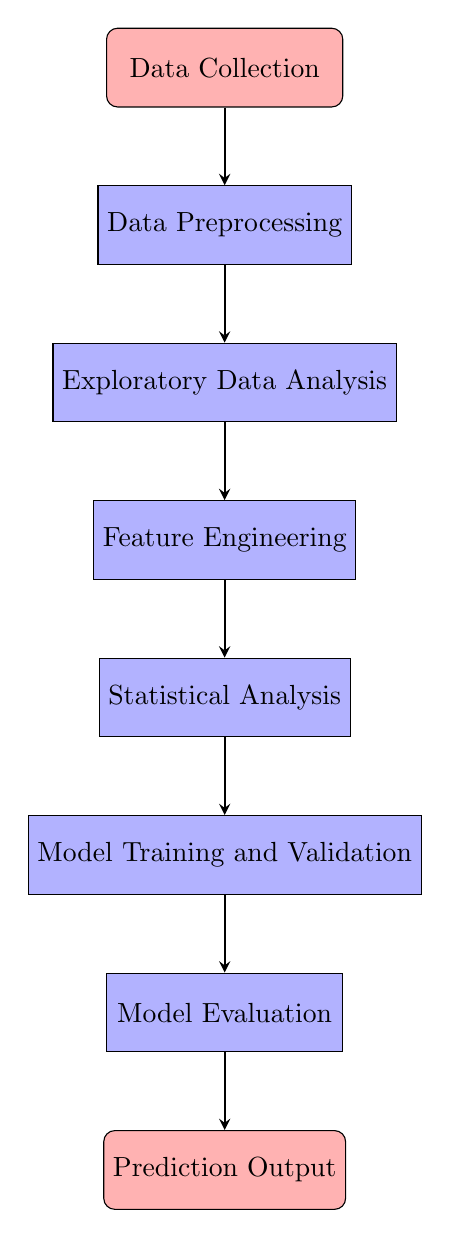
\begin{tikzpicture}[node distance=2cm]

% Nodes
\node (start) [startstop] { Data Collection};
\node (preprocessing) [process, below of=start] {Data Preprocessing};
\node (eda) [process, below of=preprocessing] {Exploratory Data Analysis};
\node (features) [process, below of=eda] {Feature Engineering};
\node (stats) [process, below of=features] {Statistical Analysis};
\node (modeling) [process, below of=stats] {Model Training and Validation};
\node (evaluation) [process, below of=modeling] {Model Evaluation};
\node (prediction) [startstop, below of=evaluation] {Prediction Output};

% Arrows
\draw [arrow] (start) -- (preprocessing);
\draw [arrow] (preprocessing) -- (eda);
\draw [arrow] (eda) -- (features);
\draw [arrow] (features) -- (stats);
\draw [arrow] (stats) -- (modeling);
\draw [arrow] (modeling) -- (evaluation);
\draw [arrow] (evaluation) -- (prediction);

\end{tikzpicture}
\end{center}
\newpage
\section{Data Collection and Preparation}
The dataset consists of 70,000 rows with 13 features, including attributes like age, gender, cholesterol levels, glucose levels, blood pressure, and lifestyle habits such as smoking and alcohol consumption. It consists of both numerical and categorical values. The target variable indicates whether a patient is having a cardiovascular disease or not(0 or 1).  
\subsection{Data Preprocessing}
Before analysis, the data underwent preprocessing to ensure its quality and reliability. Outliers in features such as age, height, systolic blood pressure (ap\_hi), and diastolic blood pressure (ap\_lo) were removed by filtering values within the 2.5th and 97.5th percentiles. After cleaning, the dataset was reduced to 60,752 entries, ensuring consistency and accuracy.

\begin{figure}[H]
\centering
\captionsetup{font=small}
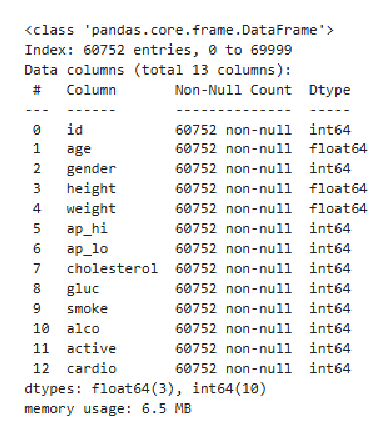
\includegraphics[width=0.5\textwidth]{dataset_cleaned.eps} 
\caption{Cleaned Dataset}
\label{fig:age_distribution}
\end{figure}

\subsection{Exploratory Data Analysis (EDA)}
EDA was conducted to understand the relationships and patterns between features. Visualizations, such as histograms and heatmaps, were used to analyze distributions and correlations. Key findings included a strong relationship between age, bmi, and map with cardiovascular disease risk.  

\begin{figure}[H]
\centering
\captionsetup{font=small}
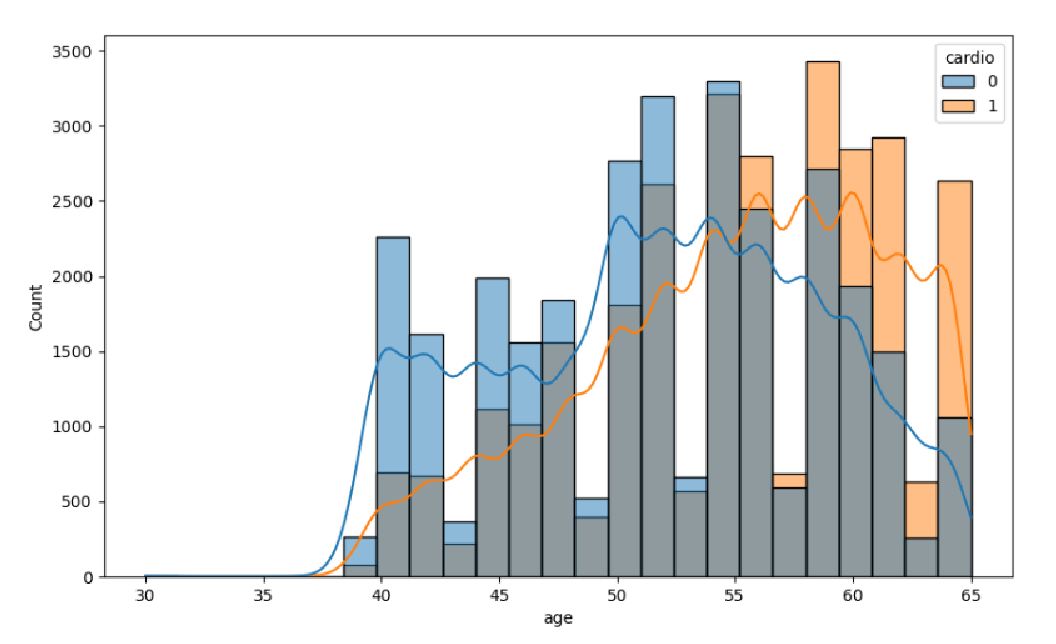
\includegraphics[width=0.35\textwidth]{graph1.eps}  % Change 'graph1.png' to your image file
\caption{Distribution of Age in the Dataset}
\label{fig:age_distribution}
\end{figure}

\begin{figure}[H]
\centering
\captionsetup{font=small}
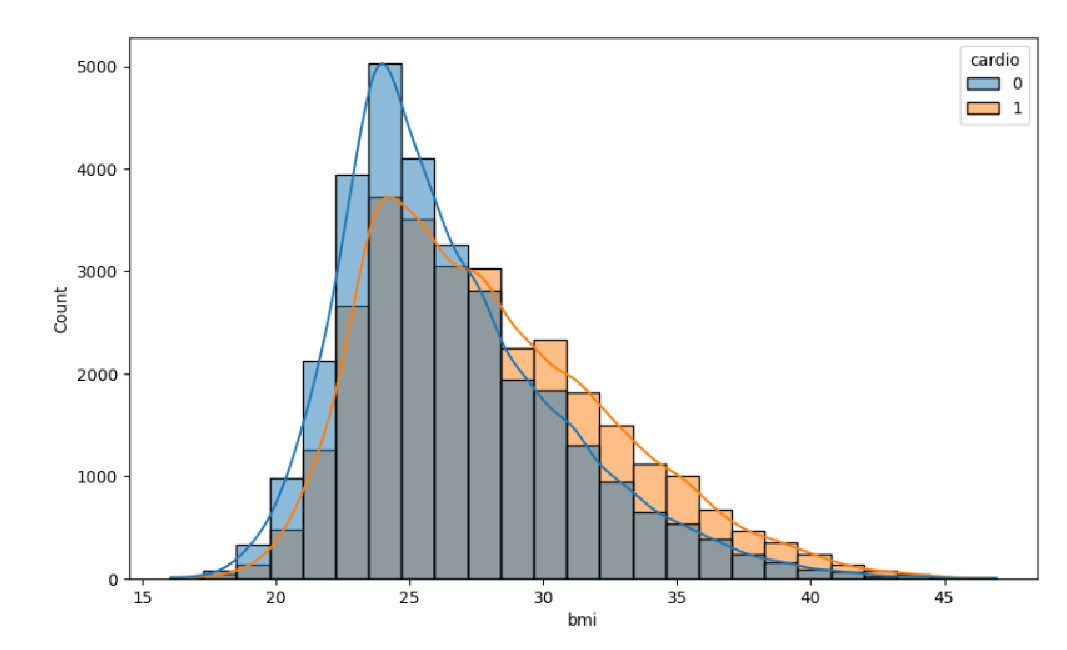
\includegraphics[width=0.35\textwidth]{graph2.eps}  % Change 'graph2.png' to your image file
\caption{Distribution of BMI in the Dataset}
\label{fig:bmi}
\end{figure}

\begin{figure}[H]
\centering
\captionsetup{font=small}
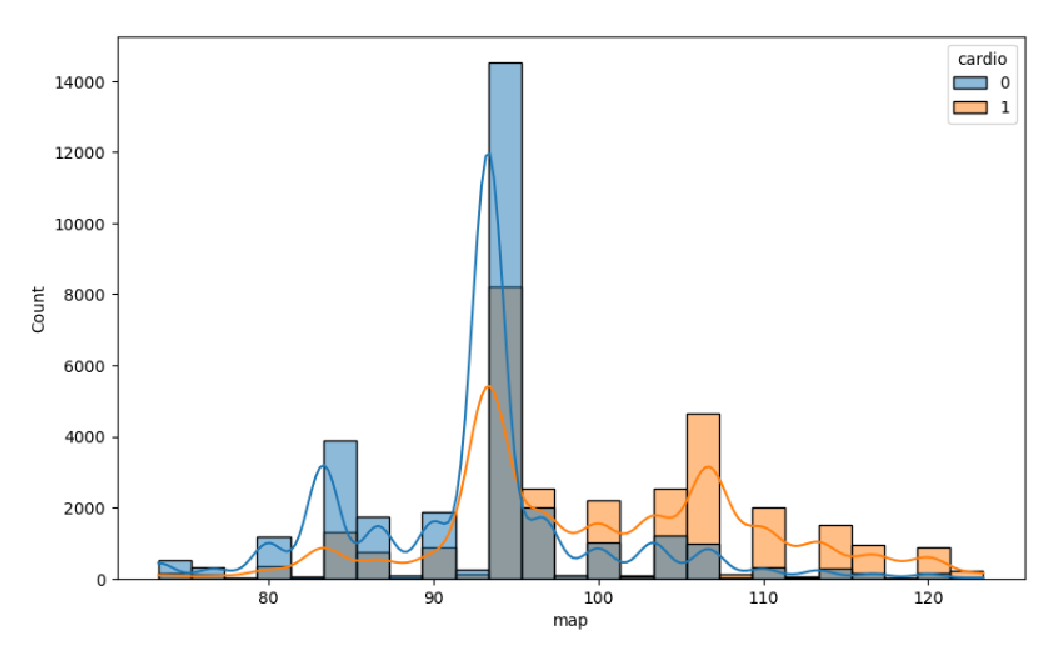
\includegraphics[width=0.35\textwidth]{graph3.eps}  % Change 'graph3.png' to your image file
\caption{Distribution of Map in the Dataset}
\label{fig:map}
\end{figure}

\subsection{Feature Engineering}
To enhance the dataset's predictive power, additional features were derived. Body Mass Index (BMI) was calculated using weight and height, and Mean Arterial Pressure (MAP) was computed using systolic and diastolic blood pressure values. MAP tells the average blood pressure in an individual during a single cardic cycle. Its says how well blood is flowing to the body’s tissues and organs. Normal map is 70 \& 100 mmHg.Categorical variables like cholesterol and glucose levels were grouped into three categories: normal, above normal, and well above normal, improving their interpretability for machine learning models.

This comprehensive data preparation process ensured a high-quality dataset for training and validating machine learning models, ultimately improving the prediction accuracy for heart disease detection.

\subsection{Correlation matrix}
 The correlation matrix is a statistical tool used to measure the strength and direction of relationships between numerical features in the dataset. For this project, the correlation matrix was visualized as a heatmap to identify patterns and highlight the most influential factors affecting cardiovascular disease.
\begin{figure}[H]
\centering
\captionsetup{font=small}
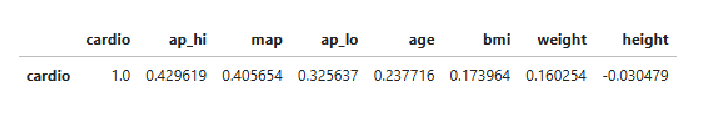
\includegraphics[width=0.75\textwidth]{correlation.eps}  
\caption{Correlation matrix between numerical features}
\label{fig:corr}
\end{figure}
As we can see from the above table, blood pressure and bmi have a strong correlation with cardiovascular disease. The correlation heatmap highlighted interactions between variables, such as the relationship between systolic and diastolic blood pressure, which informed the creation of derived features like Mean Arterial Pressure (MAP). By visualizing these relationships, the correlation matrix ensured that the most relevant features were prioritized in the predictive analysis.

\section{Statistical Analysis}
\subsection {Probabilities Related to Cholesterol Levels and Cardiovascular Disease}

\textbf{For Normal Cholesterol (\( \text{Cholesterol} = 1 \))}
\[
P(\text{Cardio} = 1 \mid \text{Cholesterol} = 1) = 0.440
\]
\[
P(\text{Cardio} = 0 \mid \text{Cholesterol} = 1) = 0.560
\]

\textbf{For Above Normal Cholesterol (\( \text{Cholesterol} = 2 \))}
\[
P(\text{Cardio} = 1 \mid \text{Cholesterol} = 2) = 0.602
\]
\[
P(\text{Cardio} = 0 \mid \text{Cholesterol} = 2) = 0.398
\]

\textbf{For Well Above Normal Cholesterol (\( \text{Cholesterol} = 3 \))}
\[
P(\text{Cardio} = 1 \mid \text{Cholesterol} = 3) = 0.765
\]
\[
P(\text{Cardio} = 0 \mid \text{Cholesterol} = 3) = 0.235
\]

\textbf{Insights}
\begin{itemize}
    \item As cholesterol levels increase, the probability of cardiovascular disease (\( P(\text{Cardio} = 1) \)) increases significantly.
    \item For normal cholesterol levels, the likelihood of no cardiovascular disease (\( P(\text{Cardio} = 0) \)) is higher.
    \item For well above normal cholesterol levels, the likelihood of cardiovascular disease (\( P(\text{Cardio} = 1) \)) dominates.
\end{itemize}


\subsection{Probabilities Related to Weight and Cardiovascular Disease}

\textbf{For Low Weight}
\[
P(\text{Cardio} = 1 \mid \text{Weight} = \text{Low}) = 0.399
\]
\[
P(\text{Cardio} = 0 \mid \text{Weight} = \text{Low}) = 0.601
\]

\textbf{For Normal Weight}
\[
P(\text{Cardio} = 1 \mid \text{Weight} = \text{Normal}) = 0.462
\]
\[
P(\text{Cardio} = 0 \mid \text{Weight} = \text{Normal}) = 0.538
\]

\textbf{For High Weight}
\[
P(\text{Cardio} = 1 \mid \text{Weight} = \text{High}) = 0.528
\]
\[
P(\text{Cardio} = 0 \mid \text{Weight} = \text{High}) = 0.472
\]

\textbf{For Very High Weight}
\[
P(\text{Cardio} = 1 \mid \text{Weight} = \text{Very High}) = 0.631
\]
\[
P(\text{Cardio} = 0 \mid \text{Weight} = \text{Very High}) = 0.369
\]

\textbf{Insights}
\begin{itemize}
    \item As weight increases, the probability of cardiovascular disease (\( P(\text{Cardio} = 1) \)) increases significantly.
    \item Conversely, the probability of no cardiovascular disease (\( P(\text{Cardio} = 0) \)) decreases with increasing weight.
\end{itemize}


\subsection{Probabilities Related to Glucose Levels and Cardiovascular Disease}

\textbf{For Normal Glucose (\( \text{Glucose} = 1 \))}
\[
P(\text{Cardio} = 1 \mid \text{Glucose} = 1) = 0.481
\]
\[
P(\text{Cardio} = 0 \mid \text{Glucose} = 1) = 0.519
\]

\textbf{For Above Normal Glucose (\( \text{Glucose} = 2 \))}
\[
P(\text{Cardio} = 1 \mid \text{Glucose} = 2) = 0.593
\]
\[
P(\text{Cardio} = 0 \mid \text{Glucose} = 2) = 0.407
\]

\textbf{For Well Above Normal Glucose (\( \text{Glucose} = 3 \))}
\[
P(\text{Cardio} = 1 \mid \text{Glucose} = 3) = 0.622
\]
\[
P(\text{Cardio} = 0 \mid \text{Glucose} = 3) = 0.378
\]

\textbf{Insights}
\begin{itemize}
    \item As glucose levels increase, the probability of cardiovascular disease (\( P(\text{Cardio} = 1) \)) increases significantly.
    \item Conversely, the probability of no cardiovascular disease (\( P(\text{Cardio} = 0) \)) decreases as glucose levels rise.
\end{itemize}

\subsection{T-test for Mean Arterial Pressure (MAP) between Smokers and Non-Smokers}

\textbf{Hypotheses}
\textbf{Null Hypothesis (Ho):} The mean MAP of smokers is equal to the mean MAP of non-smokers.  
\[
H_0: \mu_1 = \mu_2
\]

\textbf{Alternative Hypothesis (H1):} The mean MAP of smokers is not equal to the mean MAP of non-smokers.  
\[
H_1: \mu_1 \neq \mu_2
\]

Where:
\[
\mu_1 = \text{Mean of MAP for smokers}, \quad \mu_2 = \text{Mean of MAP for non-smokers}
\]

\textbf{T-test Formula}

The test statistic for a two-sample T-test is calculated as:
\[
t = \frac{\bar{x}_1 - \bar{x}_2}{\sqrt{\frac{s_1^2}{n_1} + \frac{s_2^2}{n_2}}}
\]

Where:
\begin{itemize}
    \item \(\bar{x}_1\) = Mean of MAP for smokers
    \item \(\bar{x}_2\) = Mean of MAP for non-smokers
    \item \(s_1^2\) = Variance of MAP for smokers
    \item \(s_2^2\) = Variance of MAP for non-smokers
    \item \(n_1\) = Sample size of smokers
    \item \(n_2\) = Sample size of non-smokers
\end{itemize}

\textbf{Calculated values}:
\begin{itemize}
    \item Significance level (\(\alpha\)) = 0.05
    \item Test statistic value: \(t = 5.234\)
    \item p-value: \(p = 1.663 \times 10^{-7}\)
\end{itemize}
\\
\textbf{Conclusion}

Since the p-value is much smaller than the significance level of 0.05, we reject the null hypothesis (\(H_0\)). This indicates a significant difference between the two samples in terms of Mean Arterial Pressure (MAP).

\subsection{Chi-Square Test for Association between Cholesterol Levels and Cardiovascular Disease}

\textbf{Hypotheses}
\textbf{Null Hypothesis (H0):} There is no association between cholesterol levels and cardiovascular disease. Cholesterol and cardiovascular disease are independent.
\[
H_0: P(\text{Cardio} \mid \text{Cholesterol}) = P(\text{Cardio})
\]

\textbf{Alternative Hypothesis (H1):} There is an association between cholesterol levels and cardiovascular disease. Cholesterol and cardiovascular disease are not independent.
\[
H_1: P(\text{Cardio} \mid \text{Cholesterol}) \neq P(\text{Cardio})
\]

\textbf{Chi-Square Statistic Formula}
The Chi-Square statistic is calculated as:
\[
\chi^2 = \sum \sum \frac{(O_{ij} - E_{ij})^2}{E_{ij}}
\]
Where:
\begin{itemize}
    \item \( O_{ij} \) = Observed frequency in each cell
    \item \( E_{ij} \) = Expected frequency in each cell
\end{itemize}

\textbf{Calculated values}:
\begin{itemize}
    \item Chi-Square Statistic: \( \chi^2 = 2860.95 \)
    \item p-value: \( p = 0.0 \)
    \item Degrees of Freedom: \( 2 \)
    \item Expected Frequencies: 
    \[
    \begin{bmatrix}
    23386.76 & 22641.24 \\
    4039.38 & 3910.62 \\
    3441.86 & 3332.14
    \end{bmatrix}
    \]
\end{itemize}
\\
\textbf{Conclusion}

Since the p-value is much smaller than the significance level of 0.05, we reject the null hypothesis. This suggests that variations in cholesterol levels may be linked to the presence of cardiovascular disease.

\section{Model training and Validation}
In this research, I used a dataset of 60,752 entries and 13 characteristics that included a target variable to train and verify machine learning models to predict cardiovascular illnesses. For model evaluation, the dataset was split 70:30 between training and testing. I employed three distinct algorithms: Naïve Bayes, Random Forest, and Logistic Regression.
\subsection{Training Process}
Before training the models, I applied the Standard Scaler to normalize the dataset's numerical features. Data scaling is a critical preprocessing step in machine learning, especially for algorithms like Logistic Regression and Random Forest, which can be sensitive to feature magnitude differences.

\textbf{Logistic Regression}: Since the target variable in this project has two groups (0 and 1), classification techniques were employed. Logistic Regression was chosen as the primary binary classification model due to its simplicity and effectiveness in estimating probabilities. This model uses the sigmoid function to calculate the probability of the occurrence of cardiovascular disease, providing predictions for 0 or 1. Its ease of implementation and ability to handle binary outcomes make it a suitable choice for this task.

\textbf{Random Forest}: Random Forest is an ensemble learning method that constructs a collection of decision trees during the training phase. The original dataset is divided into multiple random subsets through a technique called bagging (Bootstrap Aggregating). Each tree is trained on a different random sample of the data, and the final output is determined based on majority voting for classification tasks or averaging for regression tasks. This approach enhances prediction accuracy while reducing the risk of overfitting by leveraging the diversity among individual decision trees.

\textbf{Naïve Bayes}: Naïve Bayes is a probabilistic classifier based on Bayes' theorem, which assumes independence between the features. This assumption simplifies the computation, making it highly efficient and ideal for initial exploratory modeling. The classifier calculates the probability of each class (e.g., 0 or 1 for the target variable) and determines the class \textbf{y} that maximizes this probability. The final output is the class with the highest posterior probability, providing a straightforward yet effective approach for classification tasks.

\begin{figure}[H]
\centering
\captionsetup{font=small}
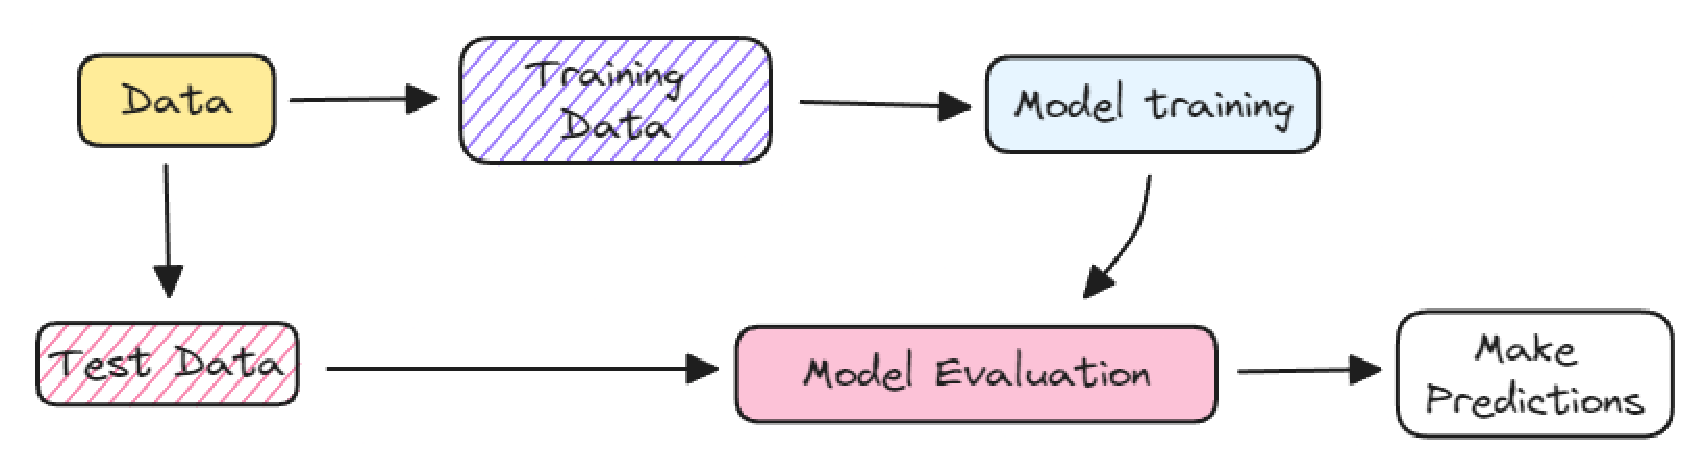
\includegraphics[width=0.75\textwidth]{ml.eps} 
\caption{Machine Learning steps}
\label{fig:ML}
\end{figure}

\subsection{Validation}
Each model was evaluated using a hold-out testing dataset, and I compared their performance based on the following metrics:

\textbf{Accuracy}: Accuracy measures how many times the model made the correct prediction out of all the predictions it made. Logistic Regression achieved the highest accuracy of 72.28\%, demonstrating its strength as a reliable binary classifier.

\textbf{ROC-AUC Score}: ROC AUC tells us how well the model can distinguish between classes across all possible classification thresholds. The ROC curve plots the true positive rate against the false positive rate. A higher AUC means the model is better at distinguishing between the classes. An AUC score of 1 means perfect performance, while an AUC of 0.5 means the model is no better than random guessing. 

\textbf{Precision and Recall}: Precision tells us how many of the items that the model predicted as positive are actually positive. Recall tells us how many of the actual positive cases the model was able to correctly identify. 
\begin{figure}[H]
\centering
\captionsetup{font=small}
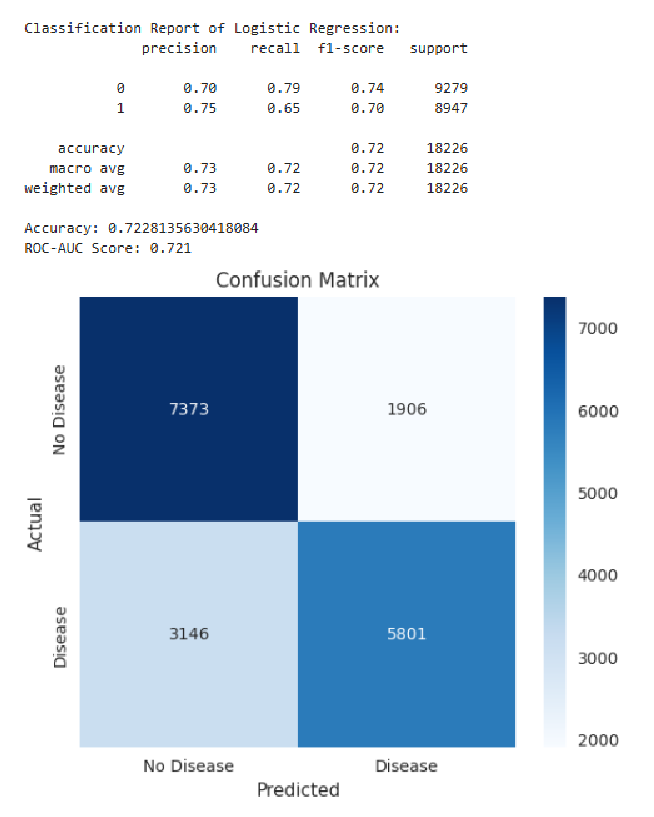
\includegraphics[width=0.5\textwidth]{classification.eps} 
\caption{Classification Report of Logistic regression}
\label{fig:classification}
\end{figure}

\section{Results}
\subsection{Machine Learning Models}
Three machine learning models—Logistic Regression, Random Forest, and Naïve Bayes—were tested for predicting cardiovascular disease. \\
\textbf{Logistic Regression}: Achieved the highest accuracy of 72.28\%, making it the most reliable model for binary classification. It performed well in predicting negative cases but had slightly lower recall for positive cases.\\
\textbf{Random Forest}: Showed balanced performance with an accuracy of 70.54\% and an ROC-AUC score of 0.753. It handled complex relationships effectively, providing consistent results.\\
\textbf{Naïve Bayes}: Had the highest ROC-AUC score, indicating strong class separation. However, its overall accuracy was slightly lower at 69.42\%, due to its assumption of feature independence.

\begin{table}[ht!]
\centering
\begin{tabular}{|c|c|c|c|c|c|}
\hline
\textbf{Model} & \textbf{Accuracy} & \textbf{Precision} & \textbf{Recall} & \textbf{ROC AUC} \\ \hline
Logistic Regression & 0.72 & 0.72 & 0.72 & 0.72  \\ \hline
Random Forest & 0.69 & 0.70 & 0.70 & 0.75 \\ \hline
Naïve Bayes & 0.71 & 0.72 & 0.71 & 0.77 \\ \hline

\end{tabular}
\caption{Performance comparison of different machine learning models}
\end{table}
\subsection{Statistical Analysis}

The Chi-Square test showed significant relationships between cardiovascular disease and features like cholesterol, glucose, and lifestyle habits.
Older age groups, higher cholesterol levels, and elevated glucose levels were strongly associated with increased cardiovascular risk. Statistical analysis further highlighted key risk factors, emphasizing the importance of features like cholesterol, mean arterial pressure, and glucose levels in predicting cardiovascular disease. These results demonstrate the effectiveness of combining machine learning and statistical techniques for health predictions.


\section{Conclusion}
This project demonstrates the importance of machine learning models and statistical analysis in predicting cardiovascular disease (CVD) based on the given dataset.

\begin{itemize}
    \item Cholesterol, Age, BMI, Glucose and MAP were found to be significant indicators of cardiovascular risk.
    \item Models like Logistic Regression, Random Forest, and Naive Bayes were effective in predicting the likelihood of heart disease, with Random Forest performing the best in distinguishing between the classes.
    \item Early prediction of heart disease using these models can help in preventive care by identifying high-risk individuals for timely intervention.
\end{itemize}

\section{Future Scope}
\begin{itemize}
    \item Use optimization techniques and ensemble methods to fine-tune hyperparameters and combine models for improved performance.
    \item Incorporating more features like family history, physical activity, and diet can enhance prediction accuracy for cardiovascular disease (CVD).
    \item  The model framework can be extended to predict other diseases like diabetes or stroke by using disease-specific features.
    \item Developing a user interface integrated with the backend model can enable real-time CVD risk predictions, making it accessible for healthcare professionals and individuals.
\end{itemize}
\newpage
\section*{References}

\begin{enumerate}
    \item Vijetha Sharma, Shrinkala Yadav, Manjari Gupta \textit{Heart Disease Prediction using Machine
Learning Techniques
}, 2020 2nd International Conference on Advances in Computing, Communication Control and Networking (ICACCCN).
    \item M. Kavitha, G. Gnaneswar, R. Dinesh, Y. Rohith Sai, R. Sai Suraj \textit{Heart Disease Prediction using Hybrid Machine
Learning Model
}, IEEE Xplore Part Number: CFP21F70-ART; ISBN: 978-1-7281-8501-9
\item Senthilkumar Mohan, Chandrasegar thirumalai, Gautam Srivastava \textit{Effective Heart Disease Prediction Using
Hybrid Machine Learning Techniques
}, Digital Object Identifier 10.1109/ACCESS.2019.2923707
\item Chintan M. Bhatt, parth Patel, Tarang Ghetia, Pier Luigi Mazzeo\textit{Effective Heart Disease Prediction Using Machine
Learning Techniques
}, https://
doi.org/10.3390/a16020088

\item V V Ramalingam, Ayantan Dandapath
\textit{Heart disease prediction using machine learning techniques: A survey
}, International Journal of Engineering \& Technology 7(2.8):684

\item Samir B Patel
\textit{Heart disease prediction using machine learning and data mining technique
}, DOI: 10.090592/IJCSC.2016.018
\item https://www.who.int/health-topics/cardiovascular-diseases
\item https://www.geeksforgeeks.org/machine-learning-models/
\item https://www.google.com/search?q=machine+learning+models\&oq=machine+learning\&
\end{enumerate}

\end{document}
